\documentclass[11pt]{article}
\usepackage{UF_FRED_paper_style}

\usepackage[utf8]{inputenc}
\usepackage[T1]{fontenc}
\usepackage[english]{babel}
\usepackage{microtype} % optional, for aesthetics
\usepackage{tabularx} % nice to have
\usepackage{booktabs} % necessary for style
% \usepackage{graphicx}
% \graphicspath{{./figures/}}
% \usepackage{listings}
% \lstset{...}

% \newcommand\code[1]{\texttt{#1}}
% \let\file\code
\usepackage{listings}
\usepackage{color}

\definecolor{dkgreen}{rgb}{0,0.6,0}
\definecolor{gray}{rgb}{0.5,0.5,0.5}
\definecolor{mauve}{rgb}{0.58,0,0.82}

\lstset{frame=tb,
  language=c,
  aboveskip=3mm,
  belowskip=3mm,
  showstringspaces=false,
  columns=flexible,
  basicstyle={\small\ttfamily},
  numbers=none,
  numberstyle=\tiny\color{gray},
  keywordstyle=\color{blue},
  commentstyle=\color{dkgreen},
  stringstyle=\color{mauve},
  breaklines=true,
  breakatwhitespace=true,
  tabsize=3
}

\onehalfspacing

\setlength{\droptitle}{-5em} %% Don't touch

% TITLE:
\title{Sistema de consulta de preços cliente servidor UDP}
\author {Lucca Augusto}

% DATE:
\date{\today}

\begin{document}

\maketitle

\section{Descrição}
Trabalho desenvolvido para a disciplina de redes do primeiro semestre de 2020.
Esse trabalho consistem em um sistema de consultas de preços de combústivel em um servidor. Os clientes podem inserir e consultar dados nesse servidor, nas consultas o servidor responde com o menor preço encontrado, nas inserções o servidor insere no arquivo de preços os dados informados. Múltiplos clientes podem ser atendidos e todos os clientes podem consultar todos os dados.

\section{Compilação e execução}
O programa é compilado pelo makefile usando o comando

\begin{lstlisting}
make
\end{lstlisting}

Para executar o programa é preciso executar primeiro o servidor e depois o cliente, já que o cliente nao conseguirá se conectar se o servidor nao estiver rodando.
Utilizando o comando seguinte é possível executar o programa em apenas uma instância do shell. Executa o servidor em background e o cliente em seguida.

\begin{lstlisting}
./servidor [-p porta] &
./cliente [-i ip] [-p porta]
\end{lstlisting}

Uma outra forma de executar é usar um shell para o servidor e um shell para o cliente.

(shell 1)
\begin{lstlisting}
./servidor [-p porta]
\end{lstlisting}


(shell 2)
\begin{lstlisting}
./cliente [-i ip] [-p porta]
\end{lstlisting}

Caso nenhum argumento seja passado aos programas, o servidor iniciará na porta padrão 8000, o cliente acessará a porta padrao 8000 com o ip padrao 127.0.0.1.


\section{Código}
O código é composto por 3 arquivos:
\begin{itemize}
\item servidor.c
\item cliente.c
\item utils.h
\end{itemize}

\subsection{servidor.c}
O arquivo servidor.c é responsável por inicializar o socket e ouvir a porta.
Após inicializar o socket, o servidor fica em espera até algum cliente se conectar na porta.
Feita a conexão, o servidor espera pela mensagem do cliente com as instruções de inserção ou pesquisa.
O servidor executa em loop até que receba um sinal de término (SIGTERM;SIGKILL).
Recebida a mensagem do cliente, a informação é decodificada e, se for uma mensagem de dados, insere os dados no arquivo. Se for uma mensagem de pesquisa, pesquisa no arquivo de acordo com as informações da mensagem e retorna o menor preço ou uma mensagem "Nenhum preço encontrado para esse combustível nesse raio." caso não exista nenhum preço de acordo com as informações fornecidas pelo cliente.

\subsubsection{Recebendo uma mensagem do cliente}
As mensagens do cliente são da forma "X id V lat long", onde X é D ou P, indicando se é uma mensagem de [D]ados ou [P]esquisa, id é um identificador da mensagem, V é um inteiro indicando o raio nas mensagens de pesquisa e o preço nas mensagens de dados, e lat e long são a latitude e longitude, respectivamente.

\subsection{cliente.c}
O arquivo cliente.c é responsavel por se conectar a porta e enviar as mensagens do usuário.
Após inicializar o socket, o cliente conecta na porta e espera pela entrada do usuário com as informações de sua mensagem.
Após o usuário entrar com as informações, o cliente envia a mensagem para o servidor, espera uma confirmação, se não foi confirmada, envia mais uma vez a mensagem.
Depois disso o cliente espera pela mensagem do servidor com a resposta de sua mensagem.

\subsubsection{Recebendo uma mensagem do servidor}
Caso o cliente tenha enviado uma mensagem de dados, o servidor responderá com uma confirmação de que os dados foram inseridos. Caso a mensagem seja de pesquisa, o servidor responderá com o menor preço, o cliente então printa na saída padrão a mensagem de resposta do servidor.

\subsection{utils.h}
Esse arquivo contém funções de IO e utéis para todos os arquivos em geral.
É responsável por fazer a inserção da mensagem do cliente no arquivo e fazer a busca de preços nesse mesmo arquivo.
Também existem funções de leitura de dados do teclado e tipificação dos dados lidos.

\section{Screenshots}

\begin{figure}[H]
    \centering
        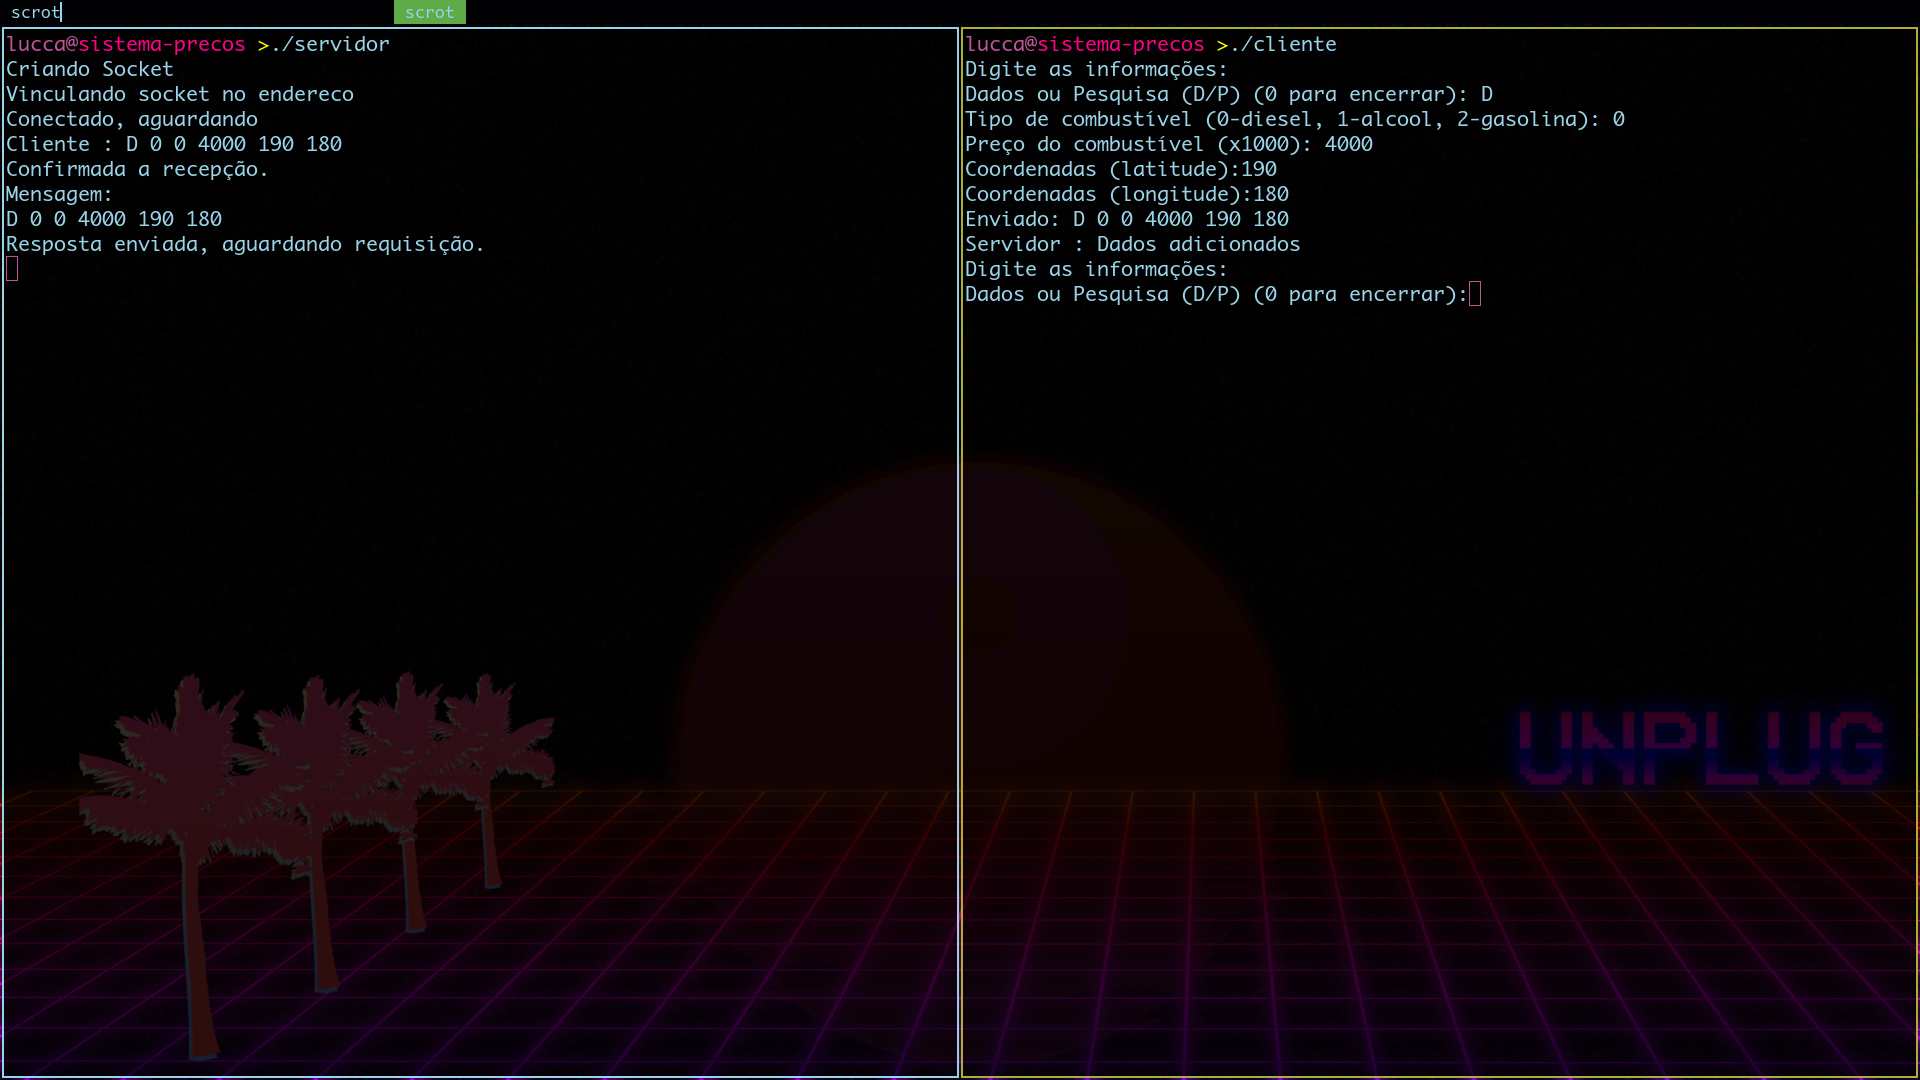
\includegraphics[scale=.2]{scrot1-sistema-precos.png}
    \caption{Screenshot mostrando a execução do programa}
    \label{fig:1}
\end{figure}
\begin{figure}[H]
    \centering
        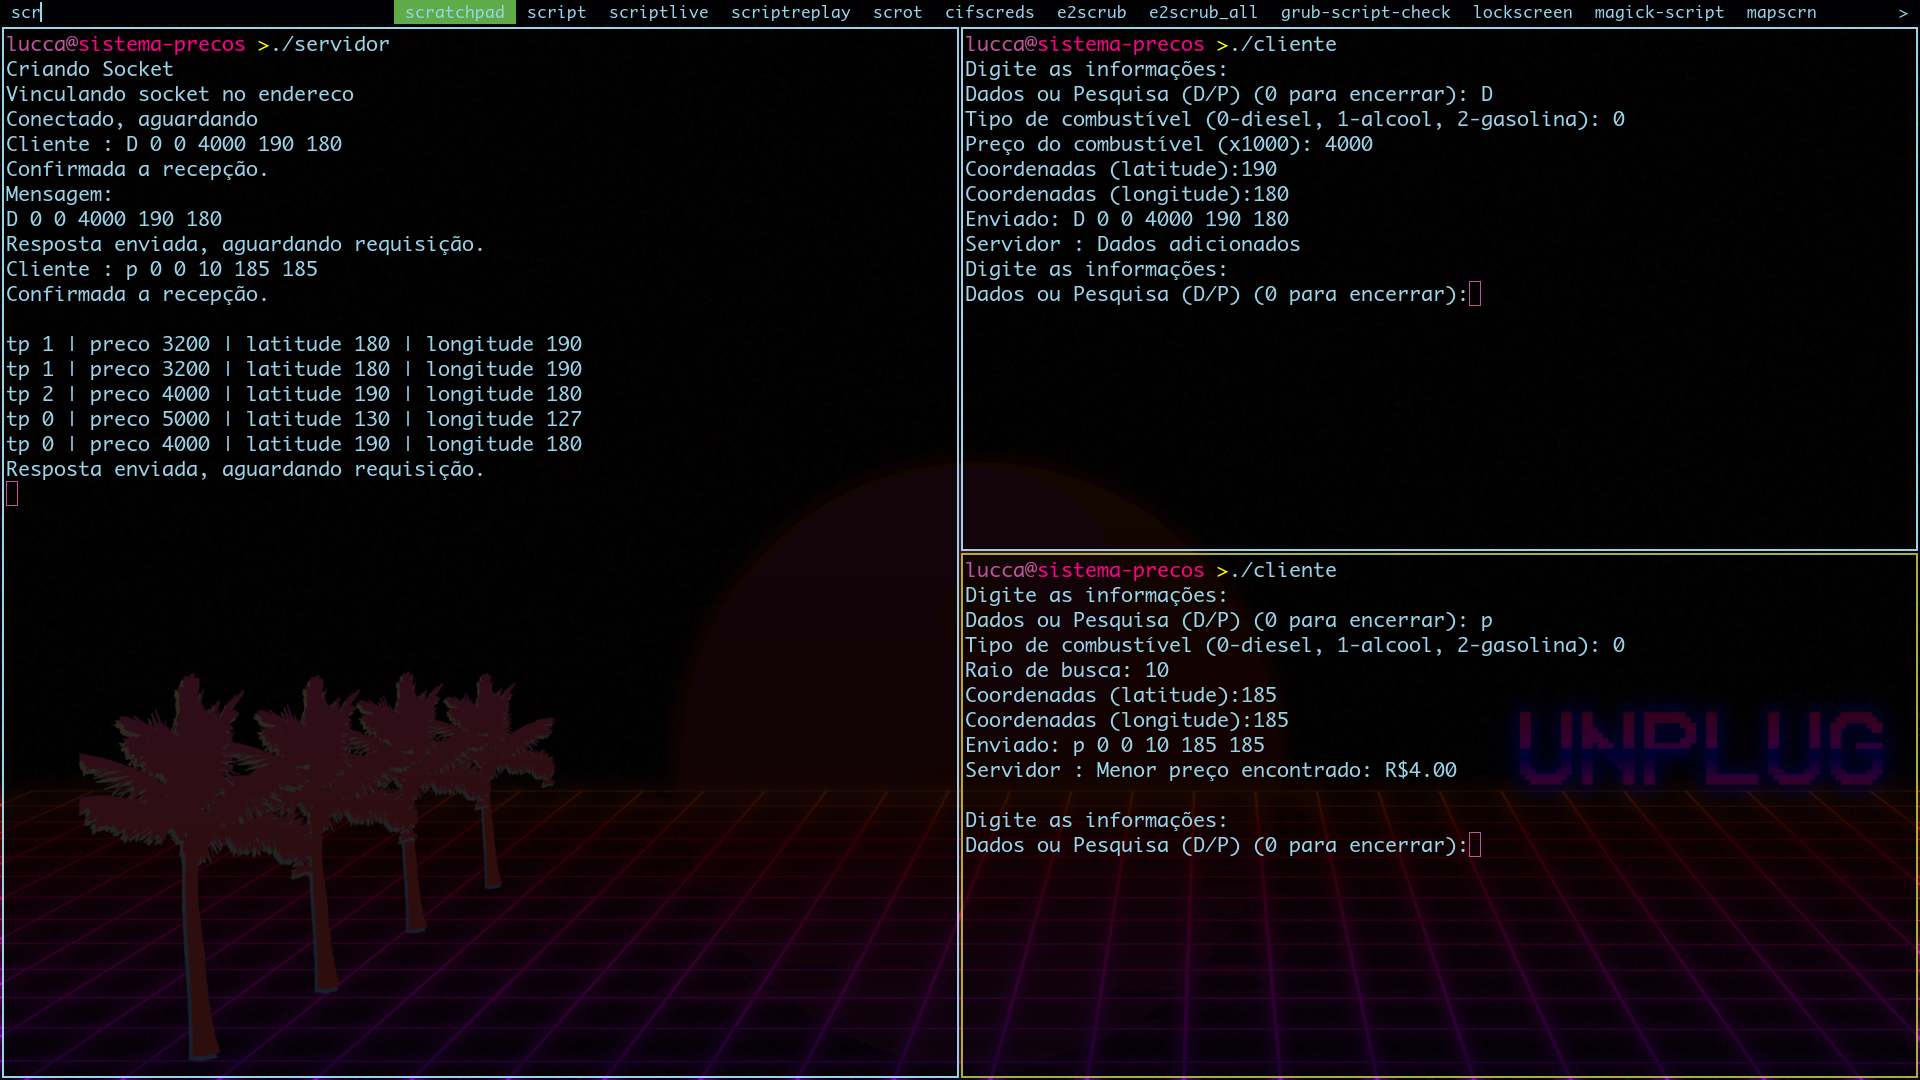
\includegraphics[scale=.2]{scrot2-sistema-precos.png}
    \caption{Screenshot mostrando a execução do programa com 2 clientes}
    \label{fig:1}
\end{figure}
\end{document}
